\section{Adaptiv}

<<<<<<< HEAD
Gennem Design sektionen, kommer vi ikke ind på den apadtive del af projektet. Dette skyldes grundet tidsmangel, at gruppen ikke nåede at implementere et adaptiv regulerings feedback. I dette afsnit, vil der forklares om adaptiv controller, og hvordan det burde være implementeret til projektet. 

\subsection{MRAC og MIT Rule}
\subsubsection{MRAC}
MRAC bruges til at designe controleren adaptivt, hvor den ændrer controller parametre, så udgangen af reference modellen og system modellen er ens. 
Herunder vises hvordan et klassisk MRAC system ser ud:


\begin{figure}[H]
	\centering
	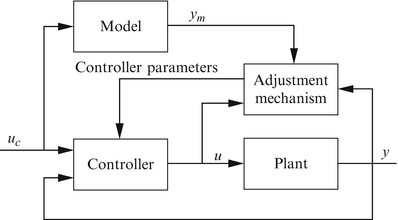
\includegraphics[width = 300pt]{figur/MRAC}
	\caption{Klassisk MRAC system}
	\label{fig:MRAC}
\end{figure}

\subsubsection{MIT Rule}
MIT rule er en måde at beregne de adjustment mechanism, som vist på figur \ref{fig:MRAC}, som skal til for at systemet opfører sig adaptiv. For at sikre stabilitet, kan den modificerede MIT rule benyttes. Dette gøres hvis reference inputtet, har store udsving, som kan gøre systemet ustabil. \\

SKAL DER MERE MED HER, EVT LIGNIGNER?

\subsection{MIAC}
Til dette projekt, skulle der have været lavet adaptiv regulering, og derigennem er der valgt, at bruge et MIAC system. Herunder vivs hvordan et klassisk MIAC system ser ud:

\begin{figure}[H]
	\centering
	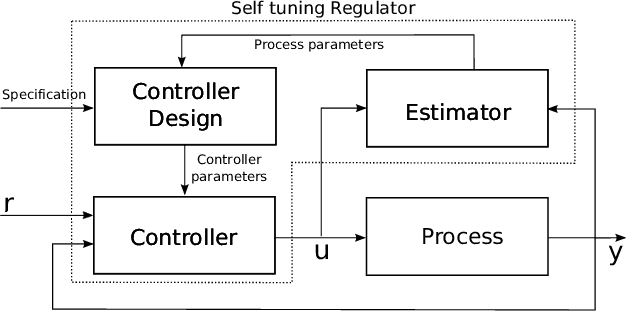
\includegraphics[width = 300pt]{figur/MIAC}
	\caption{Klassisk MIAC system}
	\label{fig:MIAC}
\end{figure}

\subsection{RLS}
Til MIAC skal derfor benyttes en regulerings mekanisme, og derigennem blev der valgt at bruge RLS algoritmen, da gruppen havde kendskab til den gennem undervisningen og den er nem at tilgå. Her skulle systemets regulerings mekanisme, laves ud fra online RLS, da systemet skulle kunne køre reel tid og derfor ikke havde et endeligt udgangssignal. 

\subsection{Implementering}
Til realiseringen af det adaptive system, var planen at indsætte RLS algoritmen i system identifications blokken, som ses på figur \ref{fig:MIAC}. Hertil skulle der laves en regulerings blok, som regulerede på K værdierne ift de valgte specs som på figur \ref{fig:Blokdiagram}.
RLS algoritmen, ville levere en thetahat som beregnes ud fra offline formlen:

\begin{figure}[H]
	\centering
	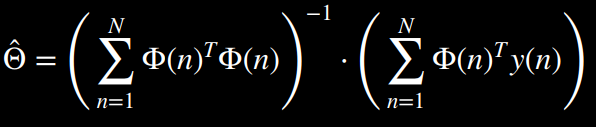
\includegraphics[width = 300pt]{figur/theta_formel}
	\caption{Formel for theta fra RLS offline blokken}
	\label{fig:theta_formel}
\end{figure}
Men da matrice beregninger, er meget tunge, omskrives formlen, da RLS skal implementeres online. 
 \begin{figure}[H]
	\centering
	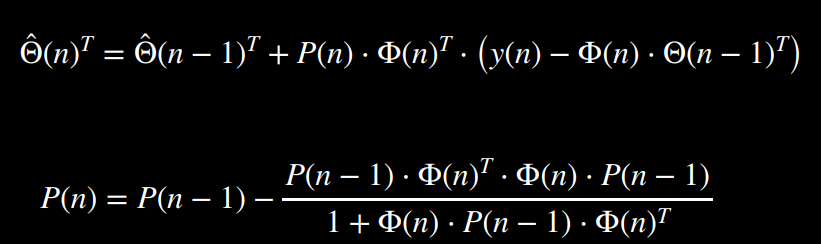
\includegraphics[width = 300pt]{figur/RLS_formel}
	\caption{Formel for theta fra RLS online blokken}
	\label{fig:RLS_formel}
\end{figure}
Hvor Phi de kendte værdier, in- og output. 
     
=======
cdscdcdfd
>>>>>>> f56296b59406512b09d5e263540e14b9446ede3f
